\section{Kombinatorika}
Notasikan $n!=n \times (n-1) \times (n-2) \times \dots \times 3 \times 2 \times 1$ (dibaca $n$ faktorial) dengan $1!=0!=1$.
\subsection{Aturan Pencacahan}
\subsection{Latihan Soal Pencacahan: Aturan Penjumlahan dan Perkalian}
\begin{enumerate}
    \item Misalkan Michie mempunyai 3 buah celana dan 4 buah baju. Berapa banyak cara Michie memilih celana dan baju yang akan dipakai ?

    \item Berapa banyak cara menyusun huruf-huruf R, A, J, I, N jika 
    \begin{enumerate}
        \item huruf pertama dimulai dari huruf hidup (vokal) 
        \item huruf pertama dimulai dari huruf mati (konsonan) 
    \end{enumerate}

    \item Sembilan orang siswa akan duduk pada 5 kursi sejajar. Ada berapa cara susunan mereka ? 
    
    \item Denny akan membentuk bilangan genap 3 angka yang angka-angkanya diambil dari 2, 3, 4, 5, 6, 7, 8. Berapa banyak bilangan yang dapat dibentuk jika : 
    \begin{enumerate}
        \item angka-angkanya boleh berulang 
        \item angka-angkanya tidak boleh berulang
    \end{enumerate}

    \item (OSK 2003) Ada berapa banyak bilangan 4-angka (digit) yang semua angkanya genap dan bukan merupakan kelipatan 2003 ?

    \item Sekumpulan orang duduk mengelilingi sebuah meja bundar. Diketahui ada 7 wanita dimana di sebelah kanan setiap wanita tersebut adalah wanita dan ada 12 wanita yang di sebelah kanan setiap wanita tersebut adalah pria. Diketahui pula bahwa 3 dari 4 pria di sebelah kanannya adalah wanita. Berapa orang yang duduk mengelilingi meja tersebut?

    \item (OSK 2015) Masing-masing kotak pada papan catur berukuran $3 \times 3$ dilabeli dengan satu angka yaitu 1, 2, atau 3. Banyaknya penomoran yang mungkin sehingga jumlah angka pada masing-masing baris dan masing-masing kolom habis dibagi 3 adalah \ldots

    \item (OSK 2023) Banyaknya bilangan 4 digit yang habis dibagi 3 dan memuat angka 6 adalah \ldots
\end{enumerate}
\subsection{Permutasi}
Permutasi $k$ unsur dari $n$ unsur adalah (urutan diperhatikan)
$$_nP_k = P_k^n = \dfrac{n!}{(n-k)!}.$$
\subsection{Latihan Soal Permutasi}
\begin{enumerate} 
    \item Sembilan orang siswa akan duduk pada 5 kursi sejajar. Ada berapa cara susunan mereka ? 
    
    \item Denny akan membentuk bilangan genap 3 angka yang angka-angkanya diambil dari 2, 3, 4, 5, 6, 7, 8. Berapa banyak bilangan yang dapat dibentuk jika : 
    \begin{enumerate}
        \item angka-angkanya boleh berulang 
        \item angka-angkanya tidak boleh berulang
    \end{enumerate}
    
    \item (OSP 2003) Empat pasang suami istri menonton pagelaran orkestra. Tempat duduk mereka harus dipisah antara kelompok suami dan kelompok istri. Untuk masing-masing kelompok disediakan 4 buah tempat duduk bersebelahan dalam satu barisan. Ada berapa banyak cara memberikan tempat duduk kepada mereka ?

    \item (OSK 2022) Di suatu ruangan terdapat 12 kursi yang disusun menjadi 3 baris. Di baris pertama, terdapat 3 kursi. Di baris kedua, terdapat 4 kursi. Di baris ketiga, terdapat 5 kursi. Jika kursi akan diduduki oleh 12 siswa termasuk Aska dan Budi. Misal banyaknya cara untuk 12 siswa menempati tempat duduk jika Aska dan Budi ada di baris pertama adalah $A$. Nilai dari $\frac{A}{8!}$ adalah \ldots

\end{enumerate}
\subsection{Kombinasi}
Kombinasi $k$ unsur dari $n$ unsur adalah (urutan tak diperhatikan)
$${n \choose k}=_nC_k = C_k^n = \dfrac{n!}{k!(n-k)!}.$$
\subsection{Latihan Soal Kombinasi}
\begin{enumerate}   
    \item  Carilah banyaknya menempatkan 3 benteng (rooks) pada papan catur $5 \times 5$ sehingga tidak ada dua catur yang dalam posisi dapat saling menyerang.

    \item Carilah banyaknya kuadrupel terurut bilangan ganjil positif $(x_1, x_2, x_3, x_4)$ yang memenuhi $x_1 + x_2 + x_3 + x_4 = 98$.

    \item Perhatikan gambar berikut. 
    
    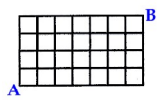
\includegraphics[width=0.2\linewidth]{assets/shortestPath.PNG} 
    
    Jika seseorang akan berjalan dari titik A ke titik B. Ada berapa banyak cara jalan terpendek yang dapat dipilihnya ?

    \item (OSK 2010) Banyaknya himpunan $X$ yang memenuhi 
    $$\{1,2,\dots,1000\} \subseteq X \subseteq \{1,2,\dots,2010\}.$$

    \item (OSP 2010) Bilangan asli enam digit $abcdef$ dengan $a > b > c \ge d > e > f$ ada sebanyak \dots
    
    \item (OSK 2017)
	Sebuah hotel mempunyai kamar bernomor 000 sampai dengan 999. Hotel tersebut menerapkan aturan aneh sebagai berikut: jika suatu kamar berisi tamu, dan sembarang dua digit nomor kamar tersebut dipertukarkan tempatnya, maka diperoleh nomor kamar yang sama atau nomor kamar yang tidak berisi tamu. Maksimal banyaknya kamar yang berisi tamu adalah \dots
\end{enumerate}
\subsection{Permutasi Siklis}
$n$ objek ditaruh mengelilingi lingkaran maka banyak cara menyusunnya adalah
$$P_{siklis} =\dfrac{n!}{n} = (n-1)!$$
\subsection{Latihan Soal Permutasi Siklis}
\begin{enumerate}
    \item (OSK 2013) Enam orang siswa akan duduk pada tiga meja bundar, dimana setiap meja akan diduduki oleh minimal satu siswa. Banyaknya cara untuk melakukan hal tersebut adalah \ldots

    \item (OSK 2015) Suatu sekolah mempunyai lima kelompok belajar siswa kelas 11. Kelompok-kelompok belajar itu berturut-turut mengirimkan 2, 2, 2, 3, dan 3 siswa untuk suatu pertemuan. Mereka akan duduk melingkar sehingga setiap siswa memiliki paling sedikit satu teman dari kelompok belajar yang sama yang duduk di sampingnya. Banyaknya cara melakukan hal tersebut adalah \ldots\\
    (Dua cara mereka duduk melingkar dianggap sama jika salah satu cara dapat diperoleh dari cara yang lain dengan suatu rotasi)
    
\end{enumerate}
\subsection{Stars and Bars}
Banyaknya solusi bulat non-negatif $(x_1,x_2,\dots,x_k)$ dari sistem persamaan $x_1+x_2+\dots+x_k=n$ adalah
$${n+k-1 \choose k-1}.$$
Banyaknya solusi bulat positif $(x_1,x_2,\dots,x_k)$ dari sistem persamaan $x_1+x_2+\dots+x_k=n$ adalah
$${n-1 \choose k-1}.$$
\subsection{Latihan Soal Stars and Bars}
\begin{enumerate}
    \item Carilah banyaknya kuadrupel terurut bilangan ganjil positif $(x_1, x_2, x_3, x_4)$ yang memenuhi $x_1 + x_2 + x_3 + x_4 = 98$.
\end{enumerate}
\subsection{Prinsip Inklusi Eksklusi}
Prinsip Inklusi (memasukkan, dari kata inklusif) Eksklusi (mengeluarkan, khusus, dari kata eksklusif) atau yang sering disingkat PIE, pada dasarnya adalah konsep dari mengurangi "kelebihan hitung" atau menambahkan "kekurangan hitung". Contohnya adalah soal himpunan yang dinyatakan dalam rumus berikut
$$|A \cup B|=|A|+|B|-|A \cap B|.$$

Untuk tiga himpunan $A,B,C$ adalah
$$|A \cup B \cup C|=|A|+|B|+|C|-|A \cap B|-|A \cap C|-|B \cap C|+|A \cap B \cap C|.$$

dan seterusnya. Lebih lengkapnya boleh mengacu ke \href{https://brilliant.org/wiki/principle-of-inclusion-and-exclusion-pie/}{https://brilliant.org/wiki/principle-of-inclusion-and-exclusion-pie/}

\subsubsection{Derangement}
Teorema ini juga bisa disebut "teorema kado silang". Bunyi teorema ini:

Misalkan $n$ adalah bilangan bulat non-negatif. Kita sebut $!n$ atau $D_n$ sebagai derangement dari $n$ yaitu banyaknya permutasi $n$ elemen berbeda sedemikian sehingga tidak ada elemen yang menempati tempatnya semula.

\textbf{Versi yang tidak terlalu abstrak:} $!n$ adalah derangement dari $n$, dimana misalkan pada sebuah pesta ulang tahun, $n$ orang saling bertukar kado (awalnya semua orang mempunyai tepat satu kado) dimana setelah bertukar kado tidak ada orang yang mendapat kado dari dirinya sendiri. Banyak kemungkinan pertukaran kado ini adalah $!n$.

Rumus umum untuk menghitung derangement adalah
$$!n = n! \left(\dfrac{1}{0!}-\dfrac{1}{1!}+\dfrac{1}{2!}-\dfrac{1}{3!}+\dfrac{1}{4!}-\dfrac{1}{5!}+\dots+(-1)^n\dfrac{1}{n!}\right).$$
\subsection{Latihan Soal Prinsip Inklusi Eksklusi}
\begin{enumerate}
    \item (OSK 2017) Terdapat enam anak, $A, B, C, D, E$ dan $F$, akan saling bertukar kado. Tidak ada yang menerima kadonya sendiri, dan kado dari $A$ diberikan kepada $B$. Banyaknya cara membagikan kado dengan cara demikian adalah \dots

    \item (OSK 2023) Banyaknya bilangan 4 digit yang habis dibagi 3 dan memuat angka 6 adalah \ldots
\end{enumerate}
\subsection{Identitas Kombinatorika}
\begin{enumerate}
    \item  ${n \choose k} = {n \choose n-k}$ dengan $k,n \in \NN_0$ dan $k \le n$.
    \item (Identitas Pascal) Untuk $n,k \in \NN_0$ berlaku ${n \choose k} + {n \choose k+1} = {n+1 \choose k+1}$
    \item (Hockey Stick Identity) Untuk $n,r\in\mathbb{N}, n>r,\sum^n_{i=r}{i\choose r}={n+1\choose r+1}$.
    \item Untuk $n,k \in \NN_0$ berlaku ${n \choose 0}+{n \choose 1} + \dots + {n \choose n} = 2^{n}$.
    \item Untuk $n,k \in \NN_0$ berlaku ${n \choose 0}+{n \choose 2} + \dots + {n \choose 2\floor{\frac{n}{2}}} = 2^{n-1}$.
    \item (Vandermonde's Identity)  $\sum_{k=0}^r\binom mk\binom n{r-k}=\binom{m+n}r$
\end{enumerate}
\subsection{Latihan Soal Identitas Kombinatorika}
\begin{enumerate}
    \item (AIME II 2000) Given that
            $\frac 1{2!17!}+\frac 1{3!16!}+\frac 1{4!15!}+\frac 1{5!14!}+\frac 1{6!13!}+\frac 1{7!12!}+\frac 1{8!11!}+\frac 1{9!10!}=\frac N{1!18!}$
            find the greatest integer that is less than $\frac N{100}$. 

        \item (AIME 1986) The polynomial $1-x+x^2-x^3+\cdots+x^{16}-x^{17}$ may be written in the form $a_0+a_1y+a_2y^2+\cdots +a_{16}y^{16}+a_{17}y^{17}$, where $y=x+1$ and the $a_i$'s are constants. Find the value of $a_2$.

        \item (AMC 10A 2016) For some particular value of $N$, when $(a+b+c+d+1)^N$ is expanded and like terms are combined, the resulting expression contains exactly $1001$ terms that include all four variables $a, b,c,$ and $d$, each to some positive power. What is $N$?
\end{enumerate}
\subsection{Binomial Newton}
Binomial Newton atau ekspansi/penjabaran binomial berfokus pada nilai koefisien setiap suku hasil penjabaran $(a+b)^n$.
$$(a+b)^n = {n \choose 0} a^nb^0 + {n \choose 1} a^{n-1}b^1+ \dots +{n \choose n}a^0b^n$$

\subsection{Latihan Soal Ekspansi Binomial Newton}
\begin{enumerate}
    \item Carilah koefisien $x^4$ dari penjabaran $(x+1)^9$

\item (OSK 2013) Koefisien $x^{2013}$ pada ekspansi
$$(1+x)^{4026}+x(1+x)^{4025}+x^2(1+x)^{4024}+\dots x^{2013}(1+x)^{2013}$$
adalah \dots

\item Jika $S=(\sqrt{71}+1)^{71}-(\sqrt{71}-1)^{71}$ adalah bilangan bulat, carilah digit terakhir dari $S$
\end{enumerate}
\subsection{Pigeon Hole Principle (PHP)}
Teorema yang dalam Bahasa Indonesia ini disebut dengan Teorema Sangkar Burung Merpati secara matematis berbunyi:
Jika ada $kn+1$ merpati dan $n$ sangkar, maka setidaknya ada satu sangkar yang berisi $k+1$ burung merpati.

Versi lebih simpelnya adalah: jika ada $n+1$ objek yang akan dibagi ke dalam $n$ buah kotak, maka setidaknya ada 1 kotak yang berisi 2 objek.

Contoh: \begin{itemize}
    \item Di dalam ruangan berisi 3 orang, pasti terdapat setidaknya 2 orang berjenis kelamin sama.
    \item Jika ada 367 orang di suatu sekolah, maka setidaknya ada dua orang diantara mereka yang tanggal lahirnya persis sama.
\end{itemize}
\subsection{Latihan Soal PigeonHole Principle}
\begin{enumerate}
\item Berapa banyak orang minimum yang harus hadir di suatu pesta sehingga dipastikan terdapat 3 orang yang lahir di bulan yang sama di pesta itu?

\item Misalkan Naruko memilih $k$ buah bilangan dari himpunan $\{1,2,3,\dots,2016\}$ secara acak. Berapakah nilai $k$ terkecil sehingga Naruko pasti bisa mendapatkan setidaknya sepasang bilangan (dari $k$ bilangan itu) yang jika dijumlahkan hasilnya 2017?

\item Suatu malam di rumah WonYoung terjadi pemadaman listrik. Karena WonYoung sangat malas, ia hanya ingin tidur dengan membawa banyak kaus kaki (hobi yang aneh :/). Ia mengambil kaus kaki dari lemari di ruangan yang sangat gelap. Lemari itu berisi 100 buah kaus kaki merah, 80 kaus kaki hijau, 60 kaus kaki biru, dan 40 kaus kaki hitam. WonYoung mengambil banyak kaus kaki tapi tidak bisa tahu warnanya. Berapa banyak kaus kaki paling sedikit yang perlu diambil sehingga dijamin terdapat setidaknya 10 pasang kaus kaki (dengan setiap pasang kaus kaki harus berwarna sama) ?

\item (OSK 2011) Di lemari hanya ada 2 macam kaos kaki yaitu kaos kaki berwarna hitam dan putih. Ali, Budi dan Candra berangkat di malam hari saat mati lampu dan mereka mengambil kaos kaki secara acak di dalam lemari dalam kegelapan. Berapa kaos kaki minimal harus mereka ambil untuk memastikan bahwa akan ada tiga pasang kaos kaki yang bisa mereka pakai ? (Sepasang kaos kaki harus memiliki warna yang sama).
    
\item Tandai satu buah kartu dengan angka 1, dua buah kartu dengan angka 2, tiga buah kartu dengan angka satu hingga lima puluh buah kartu dengan angka 50. Semua kartu tersebut dimasukkan ke dalam kotak. Berapa buah kartu minimal yang harus diambil agar dapat dipastikan terdapat sekurang-kurangnya 10 buah kartu dengan tanda angka yang sama 

\item (OSK 2016) Anak laki-laki dan anak perempuan yang berjumlah 48 orang duduk melingkar secara acak. Banyaknya minimum anak perempuan sehingga pasti ada enam anak perempuan yang duduk berdekatan tanpa diselingi anak laki-laki adalah \dots
\end{enumerate}
\subsection{Peluang}
Misalkan kita melempar sekeping koin, maka kegiatan ini disebut dengan percobaan. Hasil percobaan yang didapat biasanya adalah munculnya sisi gambar, $G$, atau munculnya sisi tulisan, $T$. Ruang contoh atau ruang sampel adalah himpunan dari \textbf{semua hasil percobaan yang mungkin} biasanya dilambangkan dengan $S$, yang dalam teori himpunan disebut dengan himpunan semesta. Pada percobaan melempar koin, ruang sampelnya adalah $\{G, T\}$ sedangkan pada percobaan melempar satu buah dadu, ruang sampelnya adalah $\{1, 2, 3, 4, 5, 6\}$. Jika $\{G, T\}$ adalah ruang sampel, maka anggota-anggota dari ruang sampel tersebut disebut titik contoh. Titik contoh dari $\{G, T\}$ adalah $G$ dan $T$. Pada percobaan melempar satu buah dadu seimbang, titik sampel yang didapat ada 6 yaitu 1, 2, 3, 4, 5, 6 sedangkan jika melempar dua buah dadu akan didapat 36 buah titik contoh, yaitu $(1, 1), (1, 2), (1, 3), \dots , (6, 6)$. 

\subsubsection{Formula Penghitungan Peluang}
Secara mudahnya, enghitung peluang bisa dengan pendekatan frekuensi, yaitu suatu percobaan yang dilakukan sebanyak $n$ kali, ternyata kejadian $A$ munculnya sebanyak $k$ kali, maka frekuensi nisbi/relatif kejadian $A$ sama dengan 
$$p(A)=\dfrac{k}{n}$$
Kalau $n$ semakin besar dan menuju tak terhingga maka nilai $p(A)$ akan cenderung konstan mendekati suatu nilai tertentu yang disebut dengan peluang munculnya kejadian $A$.

\subsection{Latihan Soal Peluang}
\begin{enumerate}
        \item (OSK 2015) Suatu dadu ditos enam kali. Probabilitas jumlah mata dadu yang muncul 9 adalah \ldots

        \item (OSK 2012) Suatu set soal terdiri dari 10 soal pilihan B atau S dan 15 soal pilihan ganda dengan 4 pilihan. Seorang siswa menjawab semua soal dengan menebak jawaban secara acak. Tentukan probabilitas ia menjawab dengan benar hanya 2 soal.

        \item (OSK 2013) Suatu partikel bergerak pada bidang Cartesius dari titik $(0, 0)$. Setiap langkah bergerak satu satuan searah sumbu $X$ positif dengan probabilitas $0.6$ atau searah sumbu $Y$ positif dengan probabilitas $0.4$. Setelah sepuluh langkah, probabilitas partikel tersebut sampai pada titik $(6,4)$ dengan melalui titik $(3,4)$ adalah \ldots
        
        \item (OSK 2012) Misalkan terdapat 5 kartu dimana setiap kartu diberi nomor yang berbeda yaitu 2, 3, 4, 5, 6. Kartu-kartu tersebut kemudian dijajarkan dari kiri ke kanan secara acak sehingga berbentuk barisan. Berapa probabilitas bahwa semua kartu yang dijajarkan dari kiri ke kanan dan ditempatkan pada tempat ke- $i$ akan lebih besar atau sama dengan $i$ untuk setiap $i$ dengan $1 \le i \le 5$ ?
        
        \item (OSK 2013) Suatu dadu ditos enam kali. Banyak cara memperoleh jumlah mata yang muncul 28 dengan tepat satu dadu muncul angka 6 adalah \dots
        
        \item (OSK 2013) Sepuluh kartu ditulis dengan angka satu sampai sepuluh (setiap kartu hanya terdapat satu angka dan tidak ada dua kartu yang memiliki angka yang sama). Kartu - kartu tersebut dimasukkan kedalam kotak dan diambil satu secara acak. Kemudian sebuah dadu dilempar. Probabilitas dari hasil kali angka pada kartu dan angka pada dadu menghasilkan bilangan kuadrat adalah \dots
        
        \item (OSK 2018) Diberikan satu koin yang tidak seimbang. Bila koin tersebut ditos satu kali, peluang muncul angka adalah $\frac{1}{4}$. Jika ditos $n$ kali, peluang muncul tepat dua angka sama dengan peluang muncul tepat tiga angka. Nilai $n$ adalah \dots
        
        \item (OSK 2017) Pada suatu kotak ada sekumpulan bola berwarna merah dan hitam yang secara keseluruhannya kurang dari 1000 bola. Misalkan diambil dua bola. Peluang terambilnya dua bola merah adalah $p$ dan peluang terambilnya dua bola hitam adalah $q$ dengan $p-q =\frac{23}{37}$. Selisih terbesar yang mungkin dari banyaknya bola merah dan hitam adalah \dots
\end{enumerate}
\subsection{Relasi Rekurensi}
Sering disebut dengan rekursif. Intinya adalah sebuah persamaan yang melibatkan barisan $a_1, a_2, \dots , a_n$ dimana untuk mendapatkan nilai $a_k$ membutuhkan suku-suku sebelumnya $a_{k-1}, a_{k-2}, \dots,$ atau $a_1$. 

Contoh paling terkenal dari persamaan rekursif adalah bilangan Fibonacci $0,1,1,2,3,5,8,13,21,\dots$ yang secara matematis didefinisikan sebagai berikut.
\begin{align*}
    F_0 &= 0, F_1 = 1\\
    F_n &= F_{n-1}+F_{n-2} \text{ untuk } n \ge 2
\end{align*}

atau yang lebih terkenal di ranah \textit{Computer Science} adalah permasalahan \textit{Tower of Hanoi} dengan persamaan rekursifnya didefinisikan sebagai berikut.
\begin{align*}
    T_1 &= 1 \\
    T_n &= 2T_{n-1}+1
\end{align*}

Untuk menyelesaikan soal relasi rekurensi, butuh manipulasi aljabar yang mumpuni sehingga tidak ada pendekatan eksplisit selain menggunakan persamaan karakteristik atau fungsi pembangkit (tidak dibahas disini) yang dijamin berhasil.

\subsubsection{Persamaan Karakteristik untuk Relasi Rekurensi Linear}
Persamaan karakteristik berikut berlaku untuk persamaan rekursif yang linear. Persamaan karakteristik berikut berguna untuk mengubah relasi rekurensi menjadi iteratif, atau persamaan berbentuk implisit. (Jadi, untuk persamaan yang bukan linear, sebagai contoh $a_n = a_{n-1}^2 + a_{n-2}$ tidak bisa dijamin selesai dengan persamaan karakteristik yang disajikan berikut).
Untuk persamaan rekursif
$$a_n = c_1a_{n-1}+c_2a_{n-2}+\dots+c_da_{n-d}$$
mempunyai persamaan karakteristik
$$x^d-c_1x^{d-1}-c_2x^{d-2}-\dots-c_dx^0=0$$

Sebagai contoh, rumus rekursif dari barisan Fibonacci di atas dapat diselesaikan menjadi 
$$x^{n}-x^{n-1}-x^{n-2}=0 \implies x^2-x-1=0$$
yang mempunyai dua akar, yaitu $x_1 = \dfrac{1+\sqrt{5}}{2}=\phi$ dan $x_2 = \dfrac{1-\sqrt{5}}{2}=1-\phi$ dimana $\phi$ adalah \textit{Golden Ratio}. Sadari bahwa setiap suku di barisan Fibonacci tersebut berbentuk $F_n = c_1x_1^n + c_2x_2^n$ (buktikan). Dengan substitusi $x_1$ dan $x_2$ serta pemilihan suku dari barisan Fibonacci (misal suku pertama dan kedua) maka akan ditemukan nilai $c_1$ dan $c_2$ sehingga pada akhirnya kita punya
$$F_n=\dfrac{\phi^n-(1-\phi)^n}{\sqrt{5}}$$
\subsection{Latihan Soal Relasi Rekurensi}
\begin{enumerate}
    \item (British) Isaac is planning a nine-day holiday. Every day he will go surfing, or water skiing, or he will rest. On any given day he does just one of these three things. He never does different water-sports on consecutive days. How many schedules are possible for the holiday?

    \item (AIME I 2006) A collection of 8 cubes consists of one cube with edge-length $k$ for each integer $k, 1 \le k \le 8.$ A tower is to be built using all 8 cubes according to the rules:
    \begin{itemize}
        \item Any cube may be the bottom cube in the tower.
        \item The cube immediately on top of a cube with edge-length $k$ must have edge-length at most $k+2.$
    \end{itemize}
    Let $T$ be the number of different towers than can be constructed. What is the remainder when $T$ is divided by 1000?

    \item (AIME I 2006) For each even positive integer $x$, let $g(x)$ denote the greatest power of 2 that divides $x.$ For example, $g(20)=4$ and $g(16)=16.$ For each positive integer $n,$ let $S_n=\sum_{k=1}^{2^{n-1}}g(2k).$ Find the greatest integer $n$ less than 1000 such that $S_n$ is a perfect square.

    \item (AIME I 2001) A mail carrier delivers mail to the nineteen houses on the east side of Elm Street. The carrier notices that no two adjacent houses ever get mail on the same day, but that there are never more than two houses in a row that get no mail on the same day. How many different patterns of mail delivery are possible?
\end{enumerate}